% This must be in the first 5 lines to tell arXiv to use pdfLaTeX, which is strongly recommended.
\pdfoutput=1
% In particular, the hyperref package requires pdfLaTeX in order to break URLs across lines.

\documentclass[11pt]{article}

% Remove the "review" option to generate the final version.
\usepackage{ACL2023}

% Standard package includes
\usepackage{times}
\usepackage{latexsym}

% For proper rendering and hyphenation of words containing Latin characters (including in bib files)
\usepackage[T1]{fontenc}

% This assumes your files are encoded as UTF8
\usepackage[utf8]{inputenc}

% This is also not strictly necessary, and may be commented out.
% However, it will improve the aesthetics of text in
% the typewriter font.
\usepackage{inconsolata}

\usepackage{lipsum, verbatim, fancyhdr, lastpage, graphicx, hyperref, amsmath, amsfonts, bm, tabularx}
\graphicspath{{./Figures/}}

\pagestyle{fancy}
\fancyhead[CO, CE]{DS 691: RnD Project}
\fancyhead[LO, LE, RO, RE]{}
\fancyfoot[CO, CE]{Page \thepage\ of \pageref{LastPage}}
\fancyfoot[LO, LE, RO, RE]{}

\title{Localizing Text Across Domains Using RARR Attribution Technique}
\author{Soumen Kumar Mondal \\
	Indian Institute of Technology Bombay \\
	\texttt{23m2157@iitb.ac.in} \\}

\begin{document}
	\maketitle
	\thispagestyle{fancy}
	\begin{abstract}
		This report explores the Retrofit Attribution using Research and Revision (RARR) model designed to enhance text localization\footnote{The code is available on GitHub: \url{https://github.com/soumenkm/RnD_Project/tree/main}} across diverse geographical domains. The primary focus is on adapting text from a reference location to a target location while maintaining factual accuracy and contextual relevance. The RARR model integrates Target Sentence Generation, Target Entity Verification, Question Generation, Search Module, Agreement Module, and Editor Module. Each component is designed to ensure that the adapted text not only aligns with the new contextual parameters but also preserves the integrity of the original information. The effectiveness of the RARR model is tested through a comprehensive dataset spanning multiple categories and locations, accompanied by a set of common questions aimed at validating the model's adaptation accuracy. This study highlights the areas of improvements and future directions for research in text localization.
	\end{abstract}
	
	\section{Introduction}
	The ability to adapt textual content accurately across different geographical and cultural contexts is an important areas of research. The Retrofit Attribution using Research and Revision (RARR) model originally proposed by \cite{gao2023rarr} is an approach designed to use for text attribution, ensuring that adapted content does not contain any factual misinformation while preserving the intent of the original text. The RARR model is adapted to enhance text localization, ensuring that adapted content not only retains the essence of the original information but also aligns seamlessly with the cultural and factual nuances of the target location.
	
	\paragraph{}The primary goal of this research is to refine the mechanisms through which text can be contextually adapted without losing its original meaning or factual accuracy. The RARR model is tested against this objective which integrates several components, including Target Sentence Generation, Target Entity Verification, Question Generation, Search Module, Agreement Module, and Editor Module. Each of these components plays an important role in the adaptation process, ensuring the text is not only accurately translated but also culturally and contextually appropriate.
	
	\paragraph{}This report presents a comprehensive evaluation of the RARR model, employing a diverse dataset that spans multiple categories and locations. The effectiveness of the model is assessed through a set of common questions designed to probe the accuracy and relevance of the adapted sentences. These questions serve as a benchmark to measure the model's capability in maintaining the integrity and accuracy of information while adapting it to different contexts.
	
	\section{Background and Related Work}
	Text localization and adaptation involve modifying textual content to suit different cultural and geographical contexts while maintaining the original message's integrity. Early efforts in this domain were focused primarily on translation and simple lexical substitution. However, recent developments have emphasized contextual and semantic appropriateness \cite{Sennrich2016, Johnson2017}. The work by \cite{Sennrich2016} introduces neural machine translation models that adapt the output by integrating target locale information directly into the training process. Similarly, \cite{Johnson2017} demonstrate the effectiveness of multilingual models in handling text adaptation by leveraging shared representations across languages.
	
	\paragraph{}The utilization of large language models for text editing and adaptation has seen considerable progress in recent years. \cite{Devlin2019}'s introduction of BERT has set a new standard for context-aware models, which has been instrumental in developing more sophisticated text adaptation techniques. Following this, GPT-3 by \cite{Brown2020} and its successors have expanded the possibilities for generating contextually relevant text across various domains, highlighting the potential for these models in automated content generation \cite{Brown2020, Radford2019}.

	\paragraph{}Despite advancements, automated text adaptation faces challenges, particularly in maintaining the nuanced differences across cultural contexts. The works of \cite{Bender2011} and \cite{Hovy2016} address these challenges by highlighting the importance of socio-cultural awareness in automated systems. Furthermore, the integration of retrieval-augmented generation as discussed by \cite{Lewis2020} has been crucial in enhancing the model's ability to utilize external knowledge bases for better text adaptation.
	
	\section{Methodology}
	We now present the method to localize the reference text in the context of target location. The detailed methodology is discussed as follows:
	
	\subsection{Target Sentence Generation}
	
	The \emph{Target Sentence Generation} module is the first component of the RARR pipeline designed to transform a reference sentence and target location into a contextually adapted target sentence. This module utilizes the provided reference sentence, such as information about a reference entity, and re-contextualizes it for a specified geographical or thematic target location as shown in Figure \ref{F:module123}. Employing few shot prompting techniques to a large language model like \emph{Mixtral 8x7b} by \cite{jiang2024mixtral}, it ensures that the generated sentence retains the factual and stylistic essence of the original input while aligning it with the new contextual parameters. 
	
	\subsection{Target Entity Verification}
	
	Following the generation of the target sentence, the \emph{Target Entity Verification} module is tasked with ensuring the accuracy and relevance of the generated content. This module scrutinizes the entities mentioned in the target sentence, verifying them with the few shot prompting in the Mixtral 8x7b model to confirm their correctness within the given context as shown in Figure \ref{F:module123}. It checks whether the factual assertions in the sentence are accurate and appropriately linked to the target location specified. This step is crucial for maintaining the credibility and reliability of the questions that would be generated later. If the generated content passes the verification process, it is accepted; otherwise, a correction is suggested with a correct target sentence.
	
	\subsection{Question Generation}
	
	The \emph{Question Generation} module operates as an attribution mechanism within the system, aimed at enhancing the overall quality and accountability of the generated target sentence. It automatically formulates questions regarding key information and assertions made in the target sentence. These questions are designed to probe the depth and accuracy of the generated content, such as querying the factual information regarding the target entity mentioned in the sentence as shown in Figure \ref{F:module123}. This module not only aids in refining the generated content through subsequent verification steps but also provides a basis for further improvements by gathering evidences against the claim.
	
	
	\begin{figure*}[tbh]
		\centering
		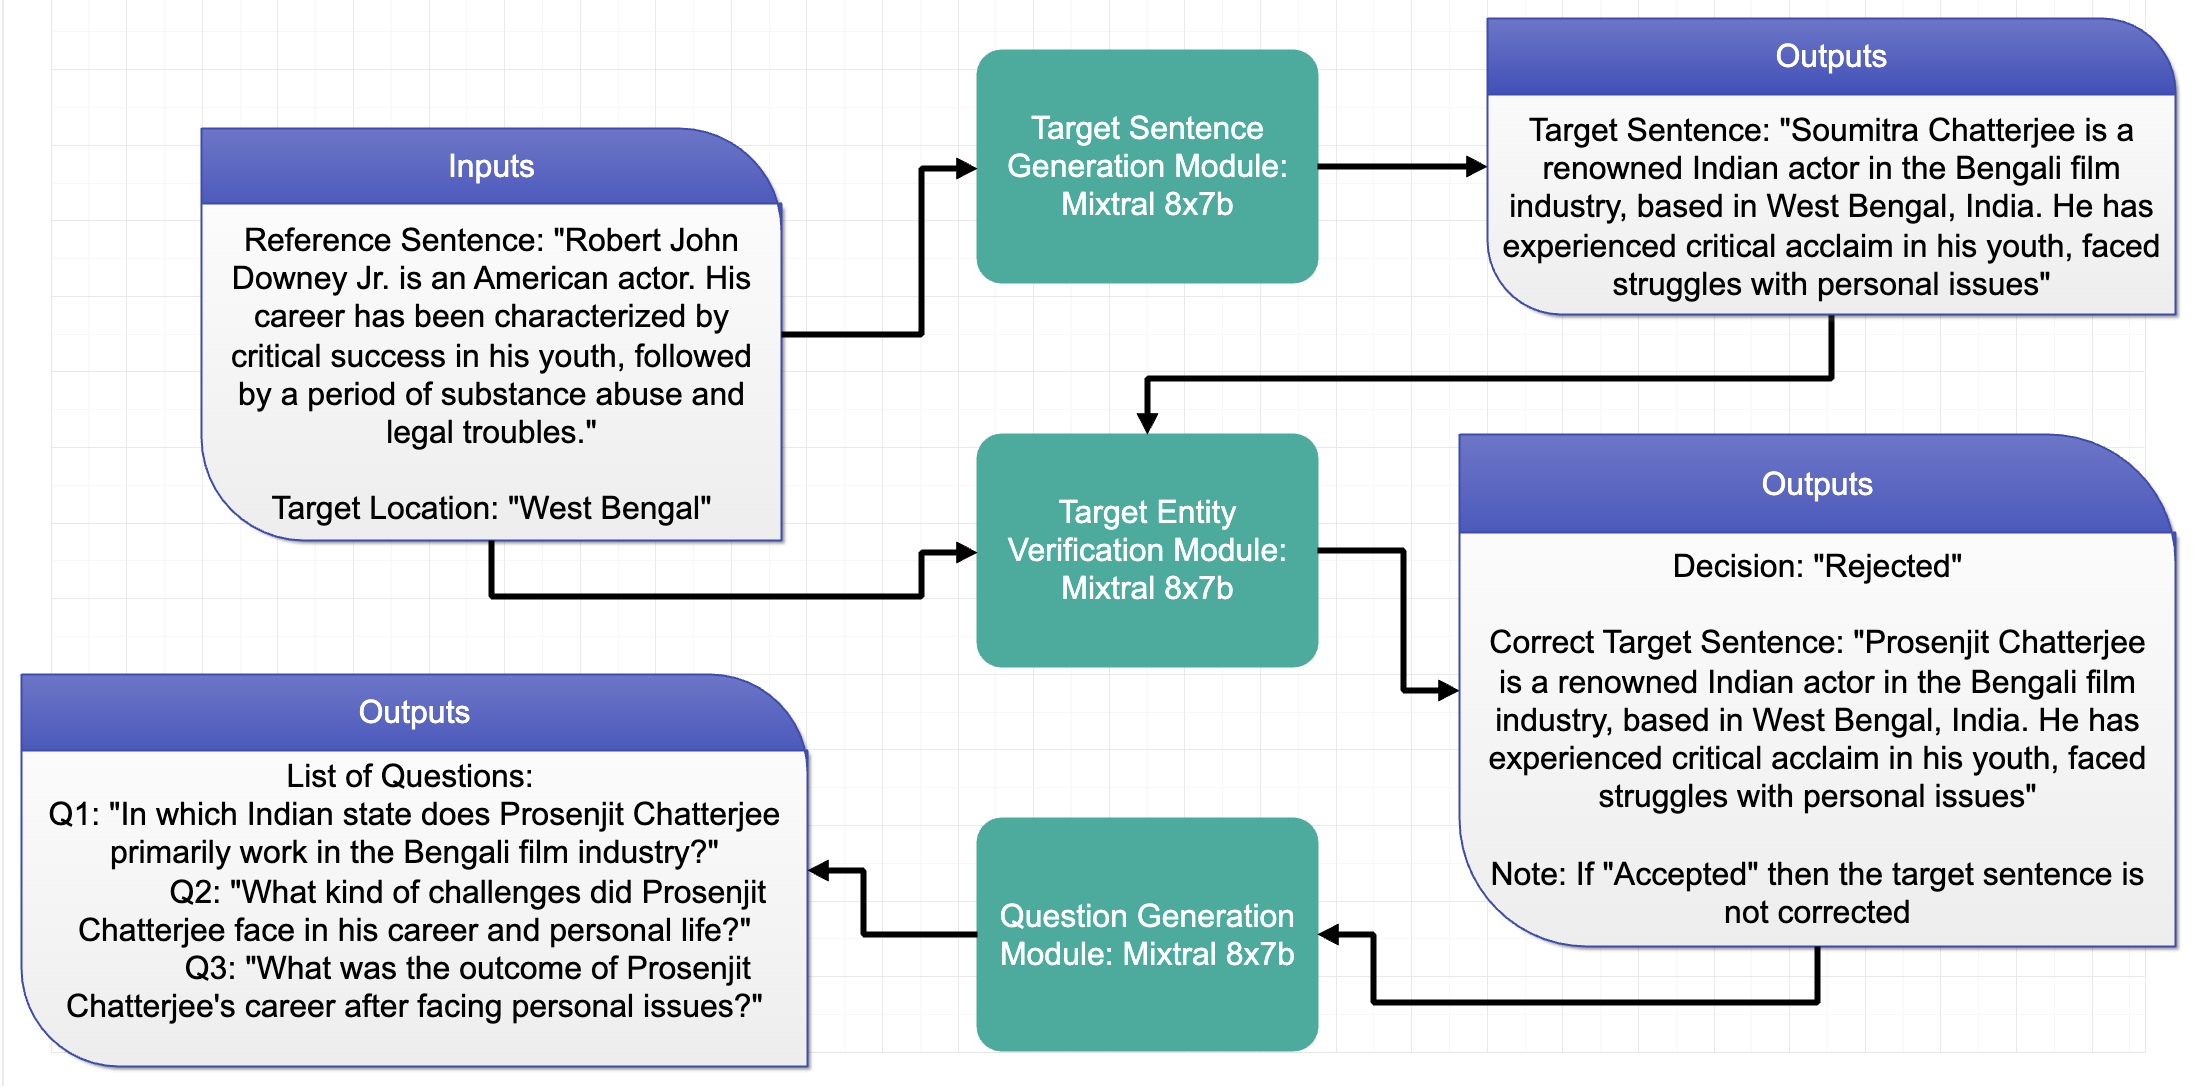
\includegraphics[width=\textwidth]{module123}
		\caption{Workflow of \emph{Target Sentence Generation}, \emph{Target Entity Verification} and \emph{Question Generation} module: The process begins with input modules that receive a reference sentence and a target location, which are then processed by the Target Sentence Generation Module (Mixtral 8x7b). The generated sentence undergoes a verification step in the Target Entity Verification Module to ensure accuracy and relevance. Questions are generated related to the entity to further probe the factual information of the content.}
		\label{F:module123}
	\end{figure*}
	
	\subsection{Search Module}
	
	The \emph{Search Module} is the key module designed to automate the process of gathering and verifying information relevant to specific questions about an entity's localized context. This module directly impacts the quality and reliability of the information extracted and subsequently used for analysis and decision-making. The Search Module integrates several key functionalities: querying an external API, scraping URLs for content, segmenting text into manageable chunks, and ranking evidence based on relevance. The module's workflow can be broken down into the following steps as shown in Figure \ref{F:module4}:
	
	\begin{enumerate}
		\item \textbf{Querying External API}: Initially, the module receives predefined questions related to the entity in focus. These questions are used to formulate queries that are sent to the Bing API, which returns a list of URLs.
		\item \textbf{URL Scraping}: Links obtained from the API are then processed for scraping. This step involves extracting textual data from the URLs, ensuring that only relevant content is retrieved. Only the top five most relevant articles are selected from the initial list provided by the Bing API to maintain focus and reduce processing load.
		\item \textbf{Chunking Text}: The scraped text is divided into manageable chunks using a sliding window approach, where the window is defined to slide over a maximum of five sentences, ensuring thorough coverage of content. From the chunked text, the top 30 evidence pieces are selected based on their relevance scores.
		\item \textbf{Ranking Evidence}: Each chunk of text is evaluated for its relevance to the original query. This is achieved using a cross-encoder model, MiniLM-L-6-V2, which scores each piece based on its semantic closeness to the query.
	\end{enumerate}
	
	The module will produce the most relevant evidence for each of the articles against a question and after passing it through a softmax layer, the best evidence for that question is retained. The above procedure is repeated for a list of questions, which then produces a list of question and best evidence pair as the consolidated output.

	\begin{figure*}[tbh]
		\centering
		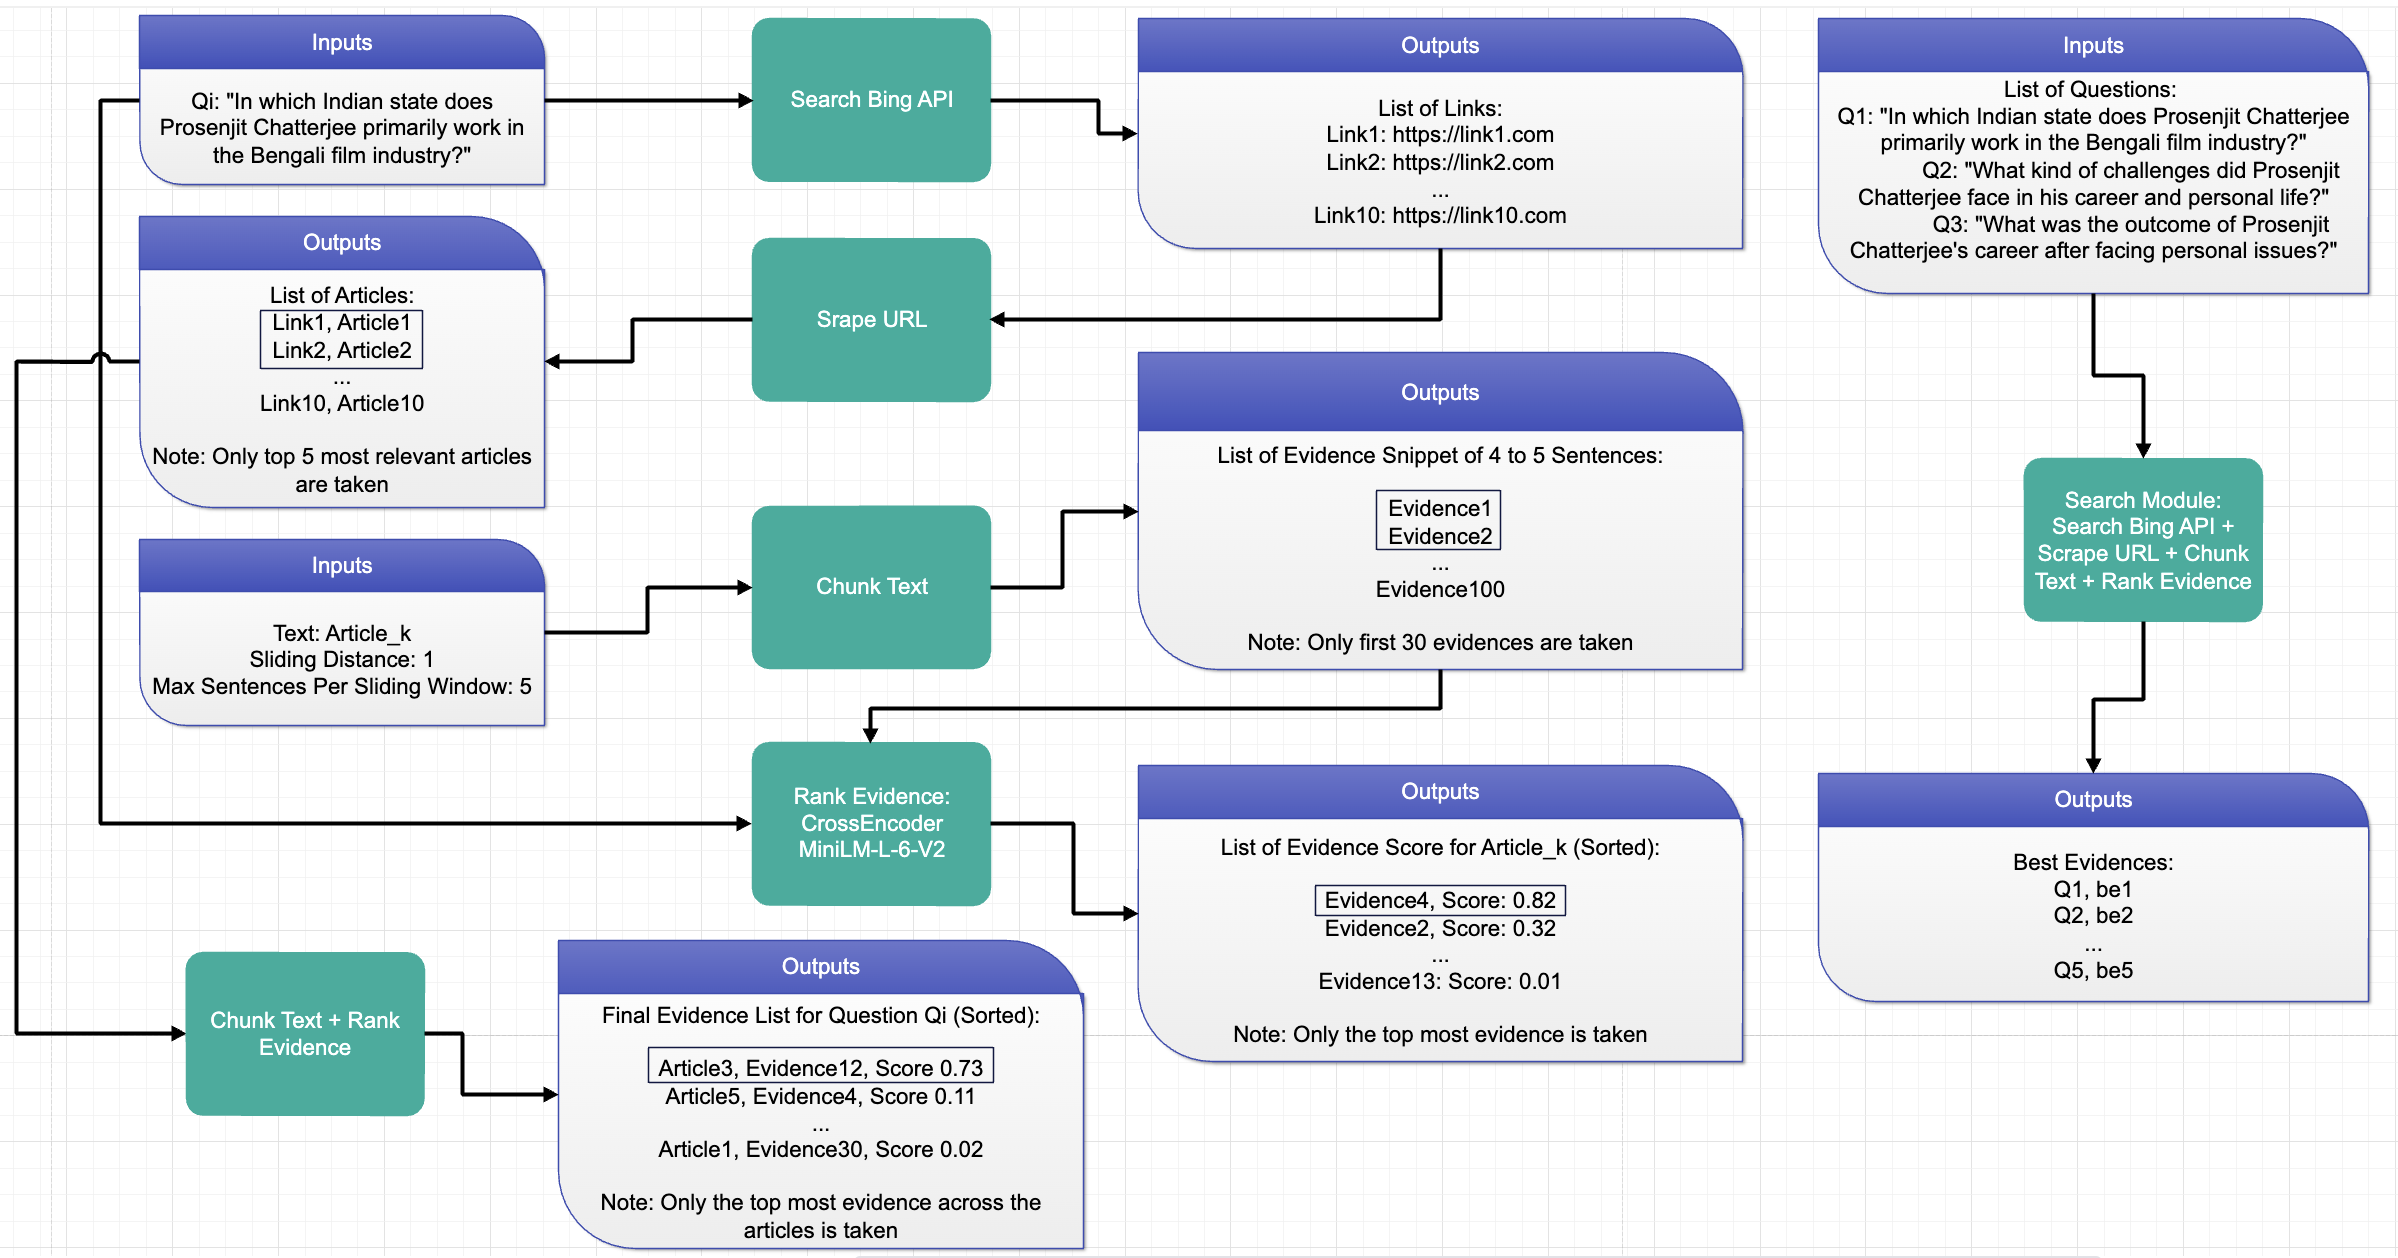
\includegraphics[width=\textwidth]{module4}
		\caption{Search Module: Initially, queries are processed through the Search Bing API, which fetches a list of relevant links. The URL scraping step then extracts text from these links, which is subsequently chunked into manageable segments. Each text segment is evaluated for relevance using the CrossEncoder model. The output of this module consists of the list of best evidence snippets that substantiate the list of questions.}
		\label{F:module4}
	\end{figure*}
	
	\subsection{Agreement Module}
	
	The \emph{Agreement Module} assesses the alignment of the generated content with verified evidence. This module utilizes the Mixtral 8x7b model to evaluate the accuracy of statements in relation to supported evidence. As shown in Figure \ref{F:module56}, the inputs to this module include the target sentence and a collection of best evidences, which are derived from prior search module. Upon receiving the inputs, the Agreement Module computes an agreement score for each piece of evidence against the target sentence. These scores are binary:
	
	\begin{itemize}
		\item \textbf{1 (Agree)}: Indicates that the evidence supports the claim made in the target sentence.
		\item \textbf{0 (Disagree)}: Indicates that the evidence contradicts the claim.
	\end{itemize}
	
	\subsection{Editor Module}
	
	Following the Agreement Module, the \emph{Editor Module} is responsible for making corrections to the target sentence based on the outcomes of the agreement assessment as shown in Figure \ref{F:module56}. This module also employs the Mixtral 8x7b model to ensure that edits maintain the factual integrity and coherence of the original content. The editor model is run sequentially for each of the question and evidence pair.
	
	\begin{enumerate}
		\item If the agreement score for a claim is \textbf{1}, the editor gate remains closed, and no edits are made to that part of the sentence.
		\item If the score is \textbf{0}, indicating a discrepancy, the sentence is modified to align with the correct factual evidence.
	\end{enumerate}
	
	The final output is an edited sentence that correctly reflects verified information, ensuring that the content is both accurate and reliable. This systematic approach allows the module to effectively manage and rectify discrepancies in generated content, thus attributing the factual information of the target sentence.
	
	\begin{figure*}[tbh]
		\centering
		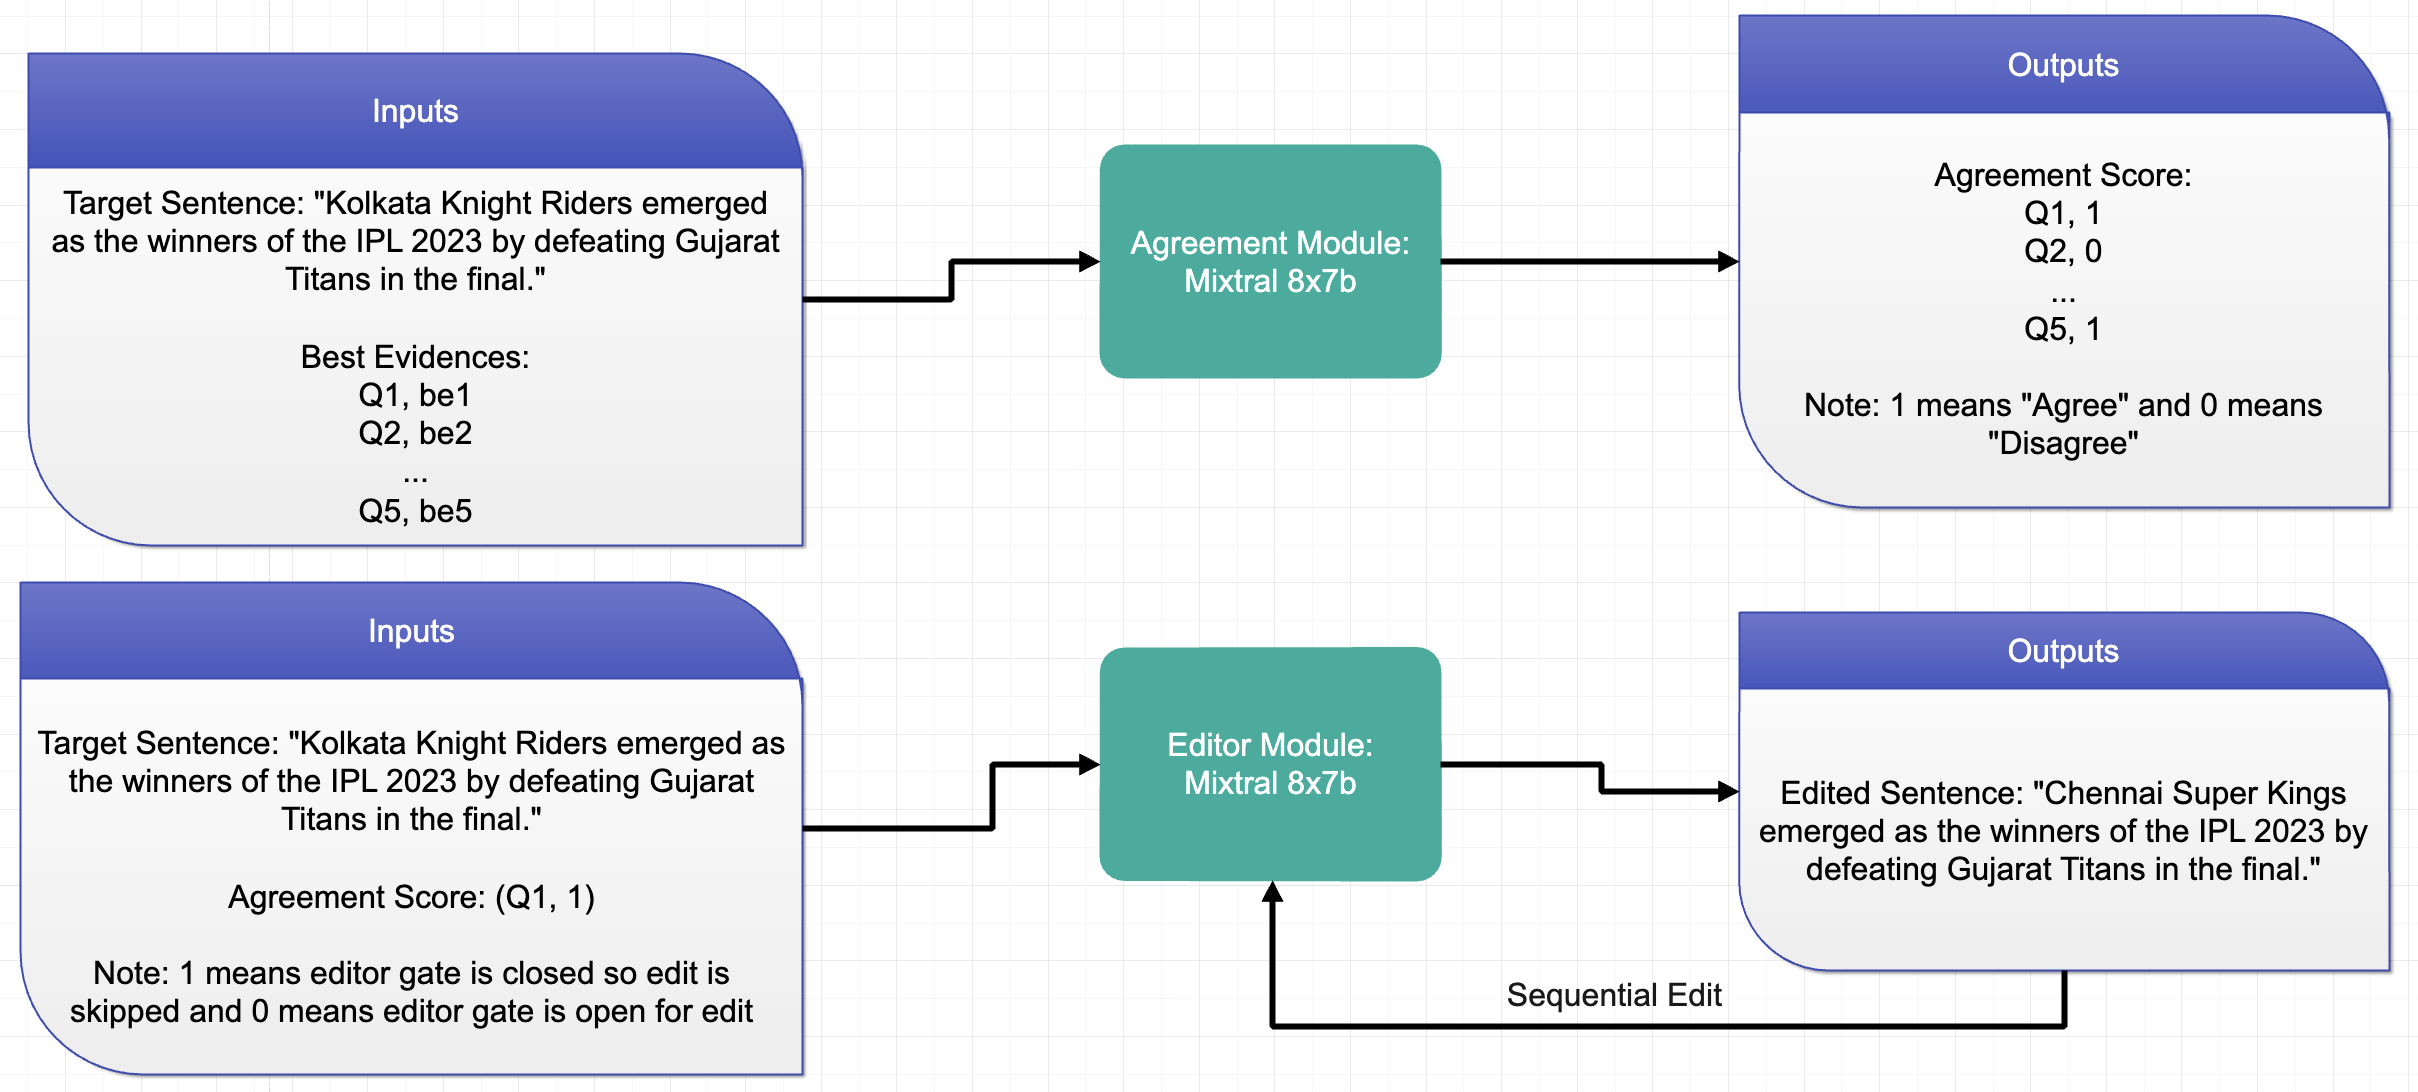
\includegraphics[width=\textwidth]{module56}
		\caption{Agreement and Editor Module: The process starts with a target sentence, which, along with gathered evidences, feeds into the Agreement Module (Mixtral 8x7b). This module assesses each evidence against the sentence and assigns an agreement score, where `1' indicates agreement (evidence supports the sentence) and `0' indicates disagreement (evidence contradicts the sentence). If any disagreement is detected (score `0'), the Editor Module is activated to revise the sentence appropriately, ensuring factual accuracy.}
		\label{F:module56}
	\end{figure*}
	
	\section{Dataset Description}
	\subsection{Reference Sentences}
	
	The dataset utilized for evaluating the RARR model comprises entries related to multiple categories across various locations globally. Each record in the dataset is structured with multiple fields including the category of the sentence, reference and target locations, entities involved and hyper locality score. This dataset facilitates a cross-domain adaptation where information are paralleled between diverse geographical locations. The dataset consists of 1000 examples spanned over 99 diverse categories which is referenced over American, European, Asian and African continents as shown in Table \ref{T:dataset}. The target location India is divided into various hyper local regions to capture the transfer of factual entity information across the domains.
	
	\subsection{Common Questions for Validation}
	
	A key component of the dataset is the set of common questions aimed at validating the model’s capability to correctly interpret and adapt information according to the specified target location. As shown in Table \ref{T:dataset}, these questions are designed to test the model's ability to extract and generate relevant information from the adapted sentences and are directly related to the incident described in the target sentence. For instance, the questions may probe for details about the incidents, such as the date, the nature of the incident, or specific outcomes.
	
	\begin{table*}[tbh]
		\centering
		\begin{tabularx}{\textwidth}{XXXX}
			\hline
			\textbf{Category, Reference and Target Location} & \textbf{Reference Sentence} & \textbf{Target Sentence} & \textbf{Common Questions} \\ \hline
			Accidents, Boston, Uttarakhand & On July 10, 2006, concrete ceiling panels and debris fell on a car traveling on the two-lane ramp connecting northbound I-93 to eastbound I-90 in South Boston, killing the passenger and injuring her husband, who was driving. & On November 12, 2023, a section of Silkyara Bend–Barkot tunnel collapsed, trapping 41 construction workers, causing injury to the workers. & (i) Can you give an instance when infrastructure failure led to people getting injured? (ii) Can you name an accident which occured due to infrastructure failure?         \\
			Actor/Actress, United States, Kerala & Dwayne Douglas Johnson, also known by his ring name the Rock, is an American actor and professional wrestler currently signed to WWE. & Mohanlal, also known by his pet name "Lalettan", is an Indian actor and producer, currently working in the Malayalam film industry. & (i) Can you give an example of an actor who professionally holds another title as well?
			(ii) Can you provide the name of an actor who is well-known in the entertainment industry by another name? \\
			\hline
		\end{tabularx}
		\caption{Comprehensive Dataset Overview for Cross-Domain Adaptation Evaluation: This dataset is used to evaluate the RARR model, featuring a diverse set of incidents and entities spread across multiple global locations. The dataset includes 1000 entries categorized into 99 types, spanning from American to Asian and African contexts. Each record is detailed with categories, reference and target locations, entities, and hyperlocal scores (not shown) to emphasize the geographical and contextual variety. Common questions associated with each record examine the model's ability to adapt and accurately attribute information in the context of the specified target location.}
		\label{T:dataset}
	\end{table*}
	
	\section{Evaluation Methods}
	The evaluation of the RARR model's output includes a critical assessment using a set of common questions designed to test the model's ability to adapt and contextualize information in target sentences. This metric focuses on determining whether the answer to each common question, based on the context of the target location, is contained within the target sentence. 
	
	\subsection{Common Question Evaluation Metric}
	
	For each target sentence, a set of predefined common questions related to the incident or entity described is used to evaluate the attribution quality of RARR model. The accuracy of the model is measured based on its ability to provide responses to these questions directly from the generated text. We use few shot prompting with GPT 3.5 to check if the answer to the common question in the context of target location is contained in the target sentence. Each response is evaluated for correctness and relevance, resulting in a binary score as follows:
	
	\begin{itemize}
		\item A score of \textbf{1} is assigned if the target sentence correctly contains the answer to the question in the context of the target location.
		\item A score of \textbf{0} is assigned if the target sentence does not contain a correct or relevant answer to the question.
	\end{itemize}
	
	\subsection{Score Calculation}
	
	For a target sentence (RARR edited target sentence output or Mixtral 8x7b output) $S^i$, the number of questions generated are $m_i$ and the list of generated questions are $\{q_j^i\}_{j=1}^{m_i}$. This list of questions when provided to GPT 3.5 as an input then it returns the binary scores as $\{A_j^i\}_{j=1}^{m_i}$. If the total number of sentences are $N$ and the total number of questions over this $N$ sentences are $Q = \sum_{i=1}^N m_i$ then the common question evaluation metric is calculated as follows:
	
	\begin{equation}
		C_{CQ} = \frac{1}{Q} \sum_{i=1}^{N} \sum_{j=1}^{m_i} A_j^i
	\end{equation}
	
	This formula aggregates the scores across all questions for all entries, providing an overall measure of the model’s effectiveness in generating contextually accurate and relevant responses. This metric is calculated for both the RARR model and the Mixtral 8x7b model to compare the effectiveness of RARR attribution against the Mixtral output which does not provide any web based attribution.
	
	\subsection{Interpretation of Results}
	
	A higher score $C_{CQ}$ for RARR indicates that the model is more effective at editing target sentences that contain accurate and relevant answers to the posed questions. This measure directly reflects the model's capability to understand and adapt the context of the reference location to the target location, ensuring the generated content is both informative and accurate. Similarly, a higher score $C_{CQ}$ for Mixtral 8x7b indicates that the model already generates the target sentence which is factually correct for the target location and the explicit attribution through RARR system may not be needed.
	
	\subsection{NLI Based Metric}
	An alternative evaluation metric could be the NLI based metric which would be calculated as:
	
	\begin{equation}
		C_{NLI} (y^i, A^i) = \frac{1}{n_i} \sum_{j=1}^{n_i} \max_k NLI(s_j^i, e_k^i)
	\end{equation}
	
	Where $S^i$ is the target sentence (RARR edited target sentence output or Mixtral 8x7b output) which consists of $n_i$ number of sentences. Therefore, $S^i = \{s_j^i\}_{j=1}^{n_i}$. The set of evidences gathered for attributing the sentence $S^i$ is given as $A^i = \{e^i_k\}_{k=1}^5$. The $NLI(s_j^i, e_k^i)$ represents the probability of $e^i_k$ entailing $s^i_j$.
	
	\section{Results and Discussion}
	
	\begin{figure*}[tbh]
		\centering
		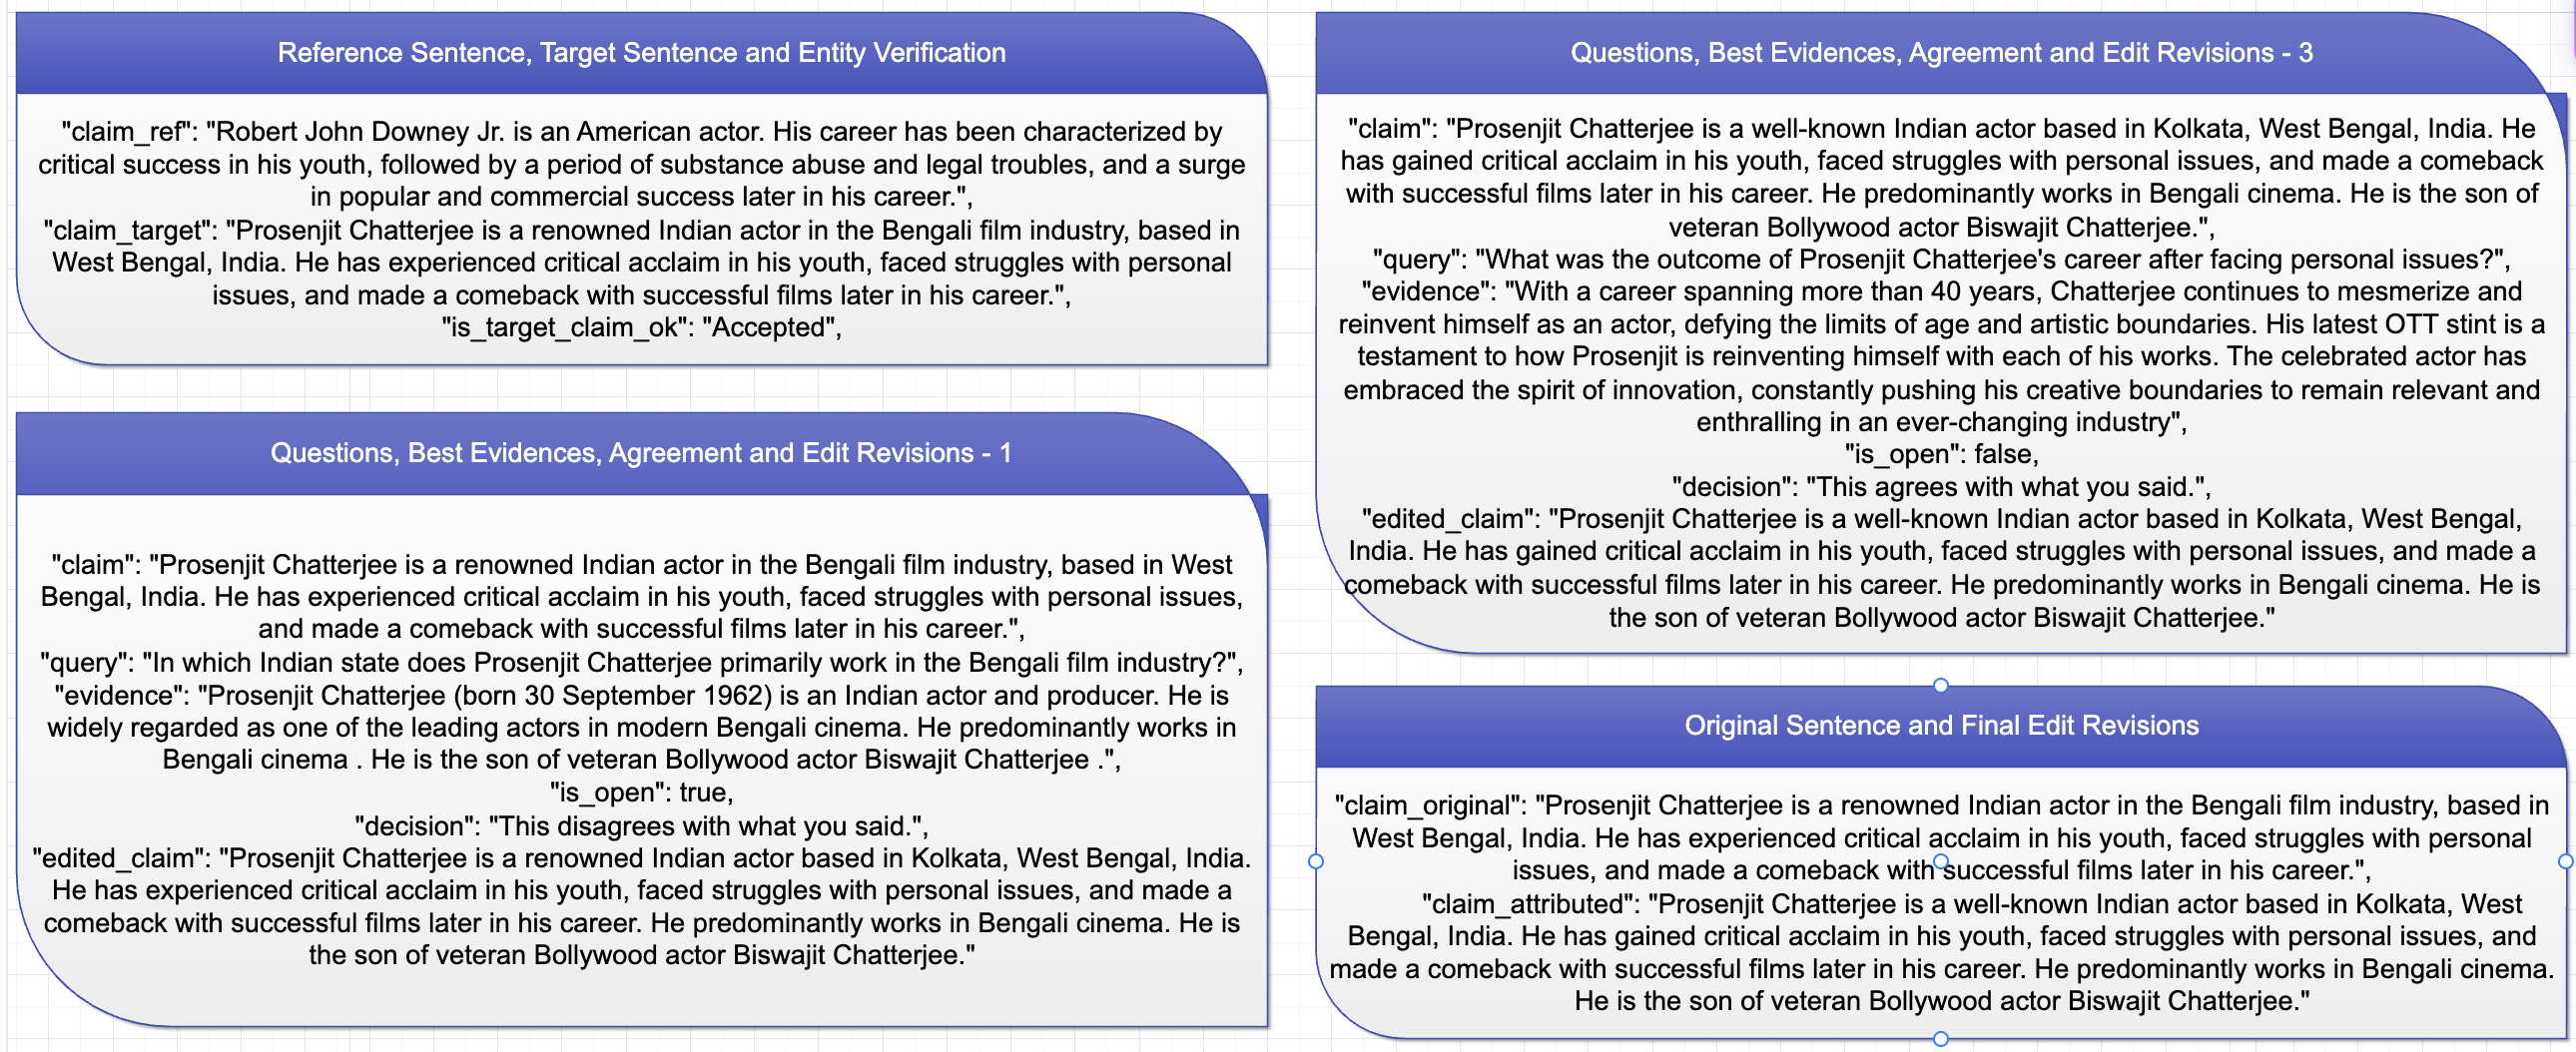
\includegraphics[width=\textwidth]{result}
		\caption{Detailed Results of RARR Model: The example illustrates the transformation of a reference sentence about an American actor into a contextually adapted sentence about an Indian actor, highlighting both syntactic and semantic adaptations. Key components shown include the initial reference and target sentences, the verification of entity accuracy, and the iterative process of question generation, evidence evaluation, and sentence editing.}
		\label{F:result}
	\end{figure*}
	
	This section presents the findings from the evaluation of the RARR model and the Mixtral 8x7b model using the common question evaluation metric outlined previously. The analysis focuses on the model's ability to generate contextually relevant and accurate responses based on the target sentences across various domains.
	
	\subsection{Discussion of Key Findings}
	
	The RARR model was tasked with generating attributed target sentences against a set of reference sentences of 200 records. The attributed target sentence from RARR model is shown in Figure \ref{F:result}. The model's performance was measured based on its ability to correctly incorporate the context of the target location into its responses based on the answers of common questions. The results from Table \ref{T: result} show that the Mixtral 8x7b outperforms RARR model in the common question evaluation metric indicating the improvement required in the RARR baseline model. However, this metric does not capture the attribution quality of the RARR which needs to be tested by NLI based metric proposed previously. It has also been observed that the RARR model is better than Mixtral 8x7b in terms of attribution but cannot outperform Mixtral 8x7b in text localization.
	
	\subsection{Ablation Studies}
	
	In this section, we examine modifications made to the original RARR pipeline to address specific issues and improve overall performance. 
	
	\begin{itemize}
		\item \textbf{Expansion of Passages for Scoring:} Initially, the RARR pipeline was configured to evaluate only the first 30 passages for scoring. To increase the coverage and relevance of the evidence assessed, this limit was removed to include \textit{all} available passages. This adjustment is intended to capture a broader spectrum of relevant information, increasing the accuracy of the context adaptation.
		
		\item \textbf{Enhancement of Embedding Quality:} The quality of embeddings derived from the MiniLM model was identified as a limiting factor in earlier implementations. To address this, we transitioned to more powerful embedding models provided by Cohere, which are designed to offer superior performance for complex language understanding tasks.
		
		\item \textbf{Revision of Editing Strategies:} Originally, edits were applied sequentially to the target text based on each piece of evidence independently. To optimize this process, we proposed aggregating all relevant evidence first and then applying a single, comprehensive edit.
	\end{itemize}
	
	These modifications are part of our ongoing efforts to refine and enhance the functionality of the RARR pipeline. However, preliminary results show that the common question evaluation metric is affected significantly due to the proposed changes.
	
	\begin{table*}[tbh]
		\centering
		\begin{tabularx}{\textwidth}{XX}
			\hline 
			\textbf{Model} & \textbf{Common Question Evaluation Metric $C_{CQ}$}  \\ \hline
			RARR Baseline & 0.5836 \\
			RARR Single Edit &0.6411 \\
			Mixtral 8x7b & 0.6439 \\
			\hline
		\end{tabularx}
		\caption{Performance Comparison of RARR and Mixtral Models Using the Common Question Evaluation Metric: The metric displayed ($C_{CQ}$) represents the proportion of common questions whose answers were correctly present in the target sentence in the context of target location. The results are averaged over 200 samples with 3 instances of target sentence generation.}
		\label{T: result}
	\end{table*}
	
	\section{Conclusions and Future Work}
	\subsection{Conclusions}
	This study has demonstrated the effectiveness of the RARR model in the field of text localization and adaptation across diverse geographical domains. The evaluation of the model using a comprehensive dataset and a set of common questions has revealed that while the RARR model performs robustly in many scenarios and attributes the factual information, the Mixtral 8x7b outperforms RARR in the common question evaluation metric.
	
	\subsection{Future Work}
	Given the insights gained from the current implementation of the RARR model, several paths for future research and development are identified:
	
	\begin{itemize}
		\item \textbf{Improving Model Robustness:} Future iterations of the RARR model will focus on enhancing the search module of RARR model indicating the use of Retrieval Augmented Models.
		
		\item \textbf{Enhanced Evaluation Metrics:} The metric currently is solely based on GPT 3.5 model. However, we can use GPT 4 model by \cite{openai2024gpt4} for the evaluation purpose.
	\end{itemize}
	
	\section*{Limitations}
	This study, while comprehensive in its approach to evaluating the RARR model, encounters several limitations that must be acknowledged:
	
	\begin{itemize}
		\item \textbf{Scope of Text Types:} The current implementation of the RARR model is primarily tested and optimized for factual text types such as news articles and informational content. It has not been extensively evaluated on creative text types like poetry or prose, where stylistic elements such as rhyme and narrative flow are crucial.
		
		\item \textbf{Subjectivity in Attribution:} Determining the necessity for attribution often involves subjective judgment, which can vary between users or contexts. The model currently lacks a robust mechanism to adapt to these subjective variations. The evaluation from LLM like GPT 3.5 is certainly a limitation of our study.
	\end{itemize}
	
	\section*{Acknowledgments}
	We extend our deepest gratitude to our academic advisor Prof. Preethi Jyothi at the Indian Institute of Technology Bombay, whose guidance and feedback have been crucial in refining the methodologies and interpretations presented in this work. Special thanks to the Amazon Research team for their collaboration and support throughout this study. Their insights and expertise have been invaluable in shaping the research and enhancing the robustness of the RARR model. We appreciate the contributions of our peer researchers and colleagues for their constructive critiques and suggestions that significantly improved the quality of this research. 
	
	% Entries for the entire Anthology, followed by custom entries
	\bibliography{ref}
	\bibliographystyle{acl_natbib}
	
\end{document}